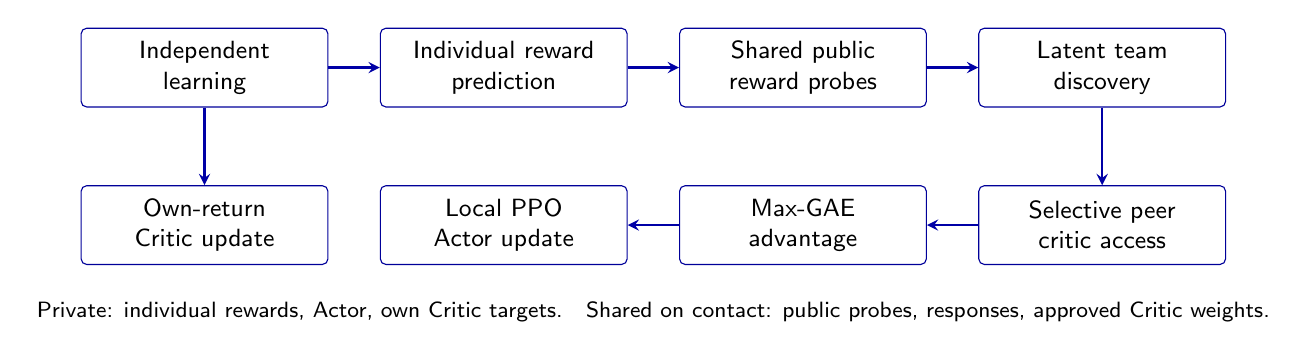
\begin{tikzpicture}[font=\sffamily\small,>=stealth,
 b/.style={draw=blue!60!black,rounded corners=2pt,align=center,minimum height=10mm,text width=29mm},
 a/.style={->,thick,blue!65!black}]
\node[b] (rl) at (0,0) {Independent\\ learning};
\node[b] (r) at (3.8,0) {Individual reward\\ prediction};
\node[b] (q) at (7.6,0) {Shared public\\ reward probes};
\node[b] (d) at (11.4,0) {Latent team\\ discovery};
\node[b] (v) at (11.4,-2) {Selective peer\\ critic access};
\node[b] (a) at (7.6,-2) {Max-GAE\\ advantage};
\node[b] (p) at (3.8,-2) {Local PPO\\ Actor update};
\node[b] (c) at (0,-2) {Own-return\\ Critic update};
\draw[a] (rl)--(r);\draw[a] (r)--(q);\draw[a] (q)--(d);
\draw[a] (d)--(v);\draw[a] (v)--(a);\draw[a] (a)--(p);
\draw[a] (rl)--(c);
\node[align=center,font=\sffamily\footnotesize] at (5.7,-3.1)
 {Private: individual rewards, Actor, own Critic targets.\quad Shared on contact: public probes, responses, approved Critic weights.};
\end{tikzpicture}
